\documentclass[border=2pt]{standalone}
\usepackage{tikz}
\usetikzlibrary{positioning}
\begin{document}
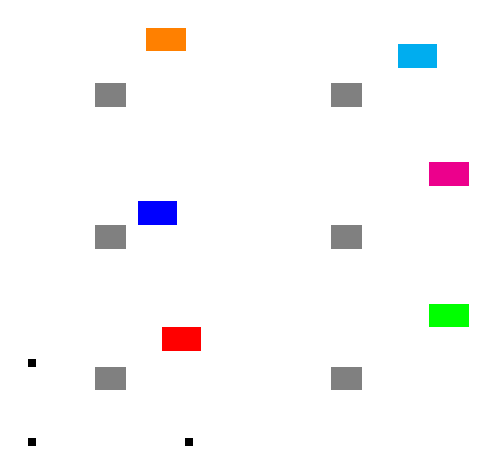
\begin{tikzpicture}[on grid,node distance=5mm and 9mm,
  base/.style={fill=gray,minimum width=4mm,minimum height=3mm,inner sep=0pt,outer sep=0pt},
  probe/.style={minimum width=5mm,minimum height=3mm,inner sep=0pt,outer sep=0pt}]
  \fill (-.5mm,-.5mm) rectangle (.5mm,.5mm);
  \fill (19.5mm,-.5mm) rectangle (20.5mm,.5mm);
  \fill (-.5mm,9.5mm) rectangle (.5mm,10.5mm);
  \node[base] (a) at (10mm,8mm) {};
  \node[base] (b) at (40mm,8mm) {};
  \node[base] (c) at (10mm,26mm) {};
  \node[base] (d) at (40mm,26mm) {};
  \node[base] (e) at (10mm,44mm) {};
  \node[base] (f) at (40mm,44mm) {};
  \node[probe,fill=red,above right=of a] {};
  \begin{scope}[node distance=8mm and 13mm]
    \node[probe,fill=green,above right=of b] {};
    \node[probe,fill=blue,node distance=3mm and 6mm,above right=of c] {};
    \node[probe,fill=magenta,above right=of d,node distance=3mm and 6mm] {};
    \begin{scope}[node distance=10mm]
      \node[probe,fill=orange,above right=of e] {};
    \end{scope}
  \end{scope}
  \node[probe,fill=cyan,above right=of f] {};
\end{tikzpicture}
\end{document}
